\section{Bethe Hessian}
\subsection{Principe}
Dans le contexte d'un SBM avec $n$ nœuds et $q$ communautés.
Chaque nœud appartient à une communauté $g_v \in \{1, \dots, q \}$
La probabilité d'une arrête entre une paire de nœud $(u, v)$ est $\mathbb{P}[A_{u,v} = 1] = p_{g_u,g_v}$.\\

L'algorithme est le même que pour la matrice d'adjacence $A$. 
Le modèle est suffisamment général pour prendre en compte un nombre arbitraire de communautés avec $q^2$ probabilités $p_{g_u,g_v}$ d’existence arrêtes différentes entre chaque communauté.\\

Il y a cependant l'apparition d'un paramètre de régularisation qu'il faut calculer au préalable.
Cependant il existe une formule fermée pour le calculer, à savoir $r= \sqrt{\frac{\langle d^2\rangle }{\langle d\rangle }- 1}$, où $\langle d\rangle$ et $\langle d^2\rangle$ sont le premier et le deuxième moment de la distribution des dégrée des nœuds dans le graphe.

L'avantage de cet opérateur linéaire par rapport à la matrice d'adjacence $A$ est, qu'avec le bon choix de $r$, l'ensemble des $q$ valeurs propres portant l'information de la structure de communauté du graphe sont négatives alors que toutes les valeurs propres du bulk de $H(r)$ sont positives.
Il suffit donc de calculer les $q$ valeurs propres négatives et s’arrêter dès que le signe change.
Grâce à ce critère discriminant, nous avons instantanément le nombre de communautés dans le graphe.
Dans le cas avec l'opérateur d'adjacence, il est impossible de faire une inférence du nombre de communauté dans la graphe.\\



Dans le cas la matrice Bethe Hessian est définie de la manière suivante:
\begin{equation}
	H(r) := (r^2 - 1)I - rA + D
\end{equation}
Où $D_{ii} = d_i \; \forall i \in V$ avec $d_i$ est le degré du nœud $i$, et $r$ est le paramètre de régularisation.\\
\subsection{Simulations}
Nous allons dans un premier temps simuler les densités spectrales des matrices Bethe hessiennes avec un SBM avec $q = 2$, $n_q=2000$, $p_{in} = 0.0035$, $p_{out} = 0.0005$.
Avec ces paramètres, le paramètre optimale est $r_{opt}\simeq2$.\\

On peut observer que lorsque $r$ est largement supérieur à $r_{opt}$, on perd la propriété où les valeurs propres contenant l'information sont négatives et celles du bulk sont positives.
Par conséquent, on ne peut plus trouver le nombre de communautés dans le graphe.
De même lorsque $r$ est largement inférieur à $r_{opt}$.

On peut voir que le comportement plus la densité spectrale en fonction de $r$ est le suivant:
\begin{itemize}
	\item plus r est grand plus la moyenne de la densité spectrale augmente
	\item plus r est proche de 0 plus les valeurs propres portant l'information se rapprochent de 0.
\end{itemize}

\begin{figure}[H]
	\begin{subfigure}{.5\textwidth}
		\centering
		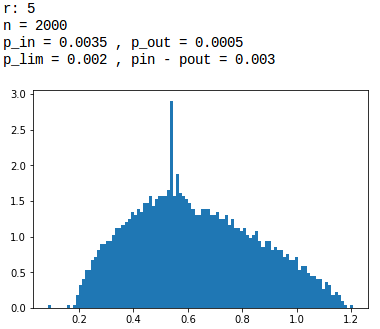
\includegraphics[scale=0.4]{static/bh_5.png}
		\label{bh5}
	\end{subfigure}
	\begin{subfigure}{.5\textwidth}
		\centering
		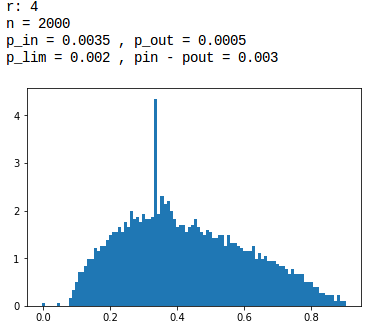
\includegraphics[scale=0.4]{static/bh_3.png}
		\label{bh3}
	\end{subfigure}
	\begin{subfigure}{.5\textwidth}
		\centering
		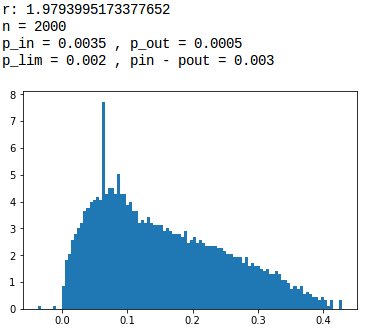
\includegraphics[scale=0.4]{static/bh_2.png}
		\label{bh2}
	\end{subfigure}
	\begin{subfigure}{.5\textwidth}
		\centering
		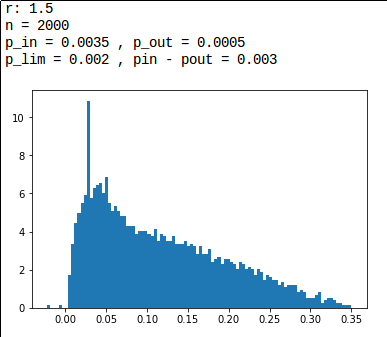
\includegraphics[scale=0.4]{static/bh_1_5.png}
		\label{bh15}
	\end{subfigure}
	\begin{subfigure}{.5\textwidth}
		\centering
		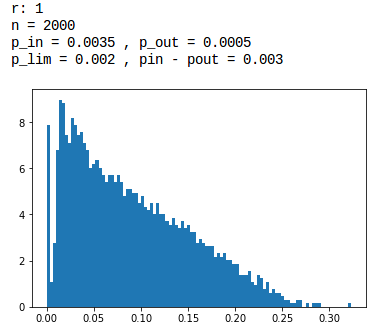
\includegraphics[scale=0.4]{static/bh_1.png}
		\label{bh1}
	\end{subfigure}
	\begin{subfigure}{.5\textwidth}
		\centering
		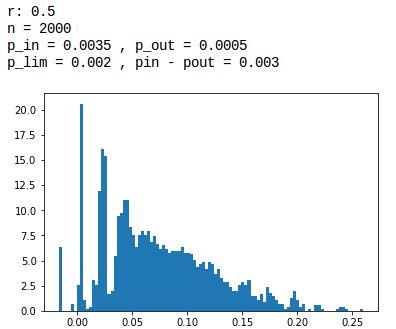
\includegraphics[scale=0.4]{static/bh_0_5.png}
		\label{bh05}
	\end{subfigure}
\end{figure}

Comme décrite dans la première partie, il faut comparer la partition obtenue de la matrice Bethe Hessian avec celle obtenue via l'algorithme ``belief propagation''.
D'après le figure 2 du papier \cite{bethe_hessian} on a:
\begin{figure}[H]
	\centering
	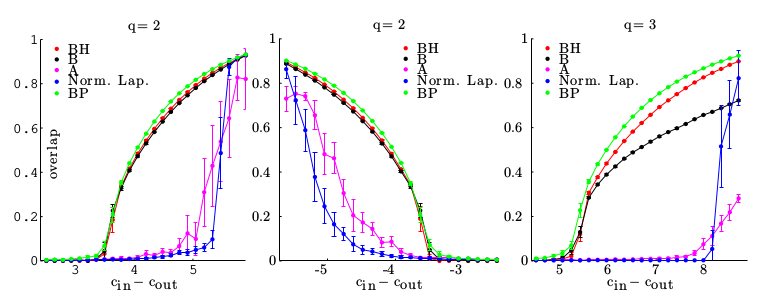
\includegraphics[scale=0.5]{static/bh_results.png}
	\caption{graphe généré à partir d'un SBM: $n=10^5$}
	\label{bhres}
\end{figure}
Ce sur cette figure il y a en ordonnée la performance de chaque algorithme via une mesure du chevauchement.
La figure à gauche correspond au cas avec 2 communautés et une structure de communauté ``assortative''.
La figure au milieu correspond aux cas avec 2 communautés et une structure de communauté ``assortative''.
La figure à droite correspond au cas avec 3 communautés et une structure de communauté ``assortative''.
